\documentclass[1p]{elsarticle_modified}
%\bibliographystyle{elsarticle-num}

%\usepackage[colorlinks]{hyperref}
%\usepackage{abbrmath_seonhwa} %\Abb, \Ascr, \Acal ,\Abf, \Afrak
\usepackage{amsfonts}
\usepackage{amssymb}
\usepackage{amsmath}
\usepackage{amsthm}
\usepackage{scalefnt}
\usepackage{amsbsy}
\usepackage{kotex}
\usepackage{caption}
\usepackage{subfig}
\usepackage{color}
\usepackage{graphicx}
\usepackage{xcolor} %% white, black, red, green, blue, cyan, magenta, yellow
\usepackage{float}
\usepackage{setspace}
\usepackage{hyperref}

\usepackage{tikz}
\usetikzlibrary{arrows}

\usepackage{multirow}
\usepackage{array} % fixed length table
\usepackage{hhline}

%%%%%%%%%%%%%%%%%%%%%
\makeatletter
\renewcommand*\env@matrix[1][\arraystretch]{%
	\edef\arraystretch{#1}%
	\hskip -\arraycolsep
	\let\@ifnextchar\new@ifnextchar
	\array{*\c@MaxMatrixCols c}}
\makeatother %https://tex.stackexchange.com/questions/14071/how-can-i-increase-the-line-spacing-in-a-matrix
%%%%%%%%%%%%%%%

\usepackage[normalem]{ulem}

\newcommand{\msout}[1]{\ifmmode\text{\sout{\ensuremath{#1}}}\else\sout{#1}\fi}
%SOURCE: \msout is \stkout macro in https://tex.stackexchange.com/questions/20609/strikeout-in-math-mode

\newcommand{\cancel}[1]{
	\ifmmode
	{\color{red}\msout{#1}}
	\else
	{\color{red}\sout{#1}}
	\fi
}

\newcommand{\add}[1]{
	{\color{blue}\uwave{#1}}
}

\newcommand{\replace}[2]{
	\ifmmode
	{\color{red}\msout{#1}}{\color{blue}\uwave{#2}}
	\else
	{\color{red}\sout{#1}}{\color{blue}\uwave{#2}}
	\fi
}

\newcommand{\Sol}{\mathcal{S}} %segment
\newcommand{\D}{D} %diagram
\newcommand{\A}{\mathcal{A}} %arc


%%%%%%%%%%%%%%%%%%%%%%%%%%%%%5 test

\def\sl{\operatorname{\textup{SL}}(2,\Cbb)}
\def\psl{\operatorname{\textup{PSL}}(2,\Cbb)}
\def\quan{\mkern 1mu \triangleright \mkern 1mu}

\theoremstyle{definition}
\newtheorem{thm}{Theorem}[section]
\newtheorem{prop}[thm]{Proposition}
\newtheorem{lem}[thm]{Lemma}
\newtheorem{ques}[thm]{Question}
\newtheorem{cor}[thm]{Corollary}
\newtheorem{defn}[thm]{Definition}
\newtheorem{exam}[thm]{Example}
\newtheorem{rmk}[thm]{Remark}
\newtheorem{alg}[thm]{Algorithm}

\newcommand{\I}{\sqrt{-1}}
\begin{document}

%\begin{frontmatter}
%
%\title{Boundary parabolic representations of knots up to 8 crossings}
%
%%% Group authors per affiliation:
%\author{Yunhi Cho} 
%\address{Department of Mathematics, University of Seoul, Seoul, Korea}
%\ead{yhcho@uos.ac.kr}
%
%
%\author{Seonhwa Kim} %\fnref{s_kim}}
%\address{Center for Geometry and Physics, Institute for Basic Science, Pohang, 37673, Korea}
%\ead{ryeona17@ibs.re.kr}
%
%\author{Hyuk Kim}
%\address{Department of Mathematical Sciences, Seoul National University, Seoul 08826, Korea}
%\ead{hyukkim@snu.ac.kr}
%
%\author{Seokbeom Yoon}
%\address{Department of Mathematical Sciences, Seoul National University, Seoul, 08826,  Korea}
%\ead{sbyoon15@snu.ac.kr}
%
%\begin{abstract}
%We find all boundary parabolic representation of knots up to 8 crossings.
%
%\end{abstract}
%\begin{keyword}
%    \MSC[2010] 57M25 
%\end{keyword}
%
%\end{frontmatter}

%\linenumbers
%\tableofcontents
%
\newcommand\colored[1]{\textcolor{white}{\rule[-0.35ex]{0.8em}{1.4ex}}\kern-0.8em\color{red} #1}%
%\newcommand\colored[1]{\textcolor{white}{ #1}\kern-2.17ex	\textcolor{white}{ #1}\kern-1.81ex	\textcolor{white}{ #1}\kern-2.15ex\color{red}#1	}

{\Large $\underline{12n_{0117}~(K12n_{0117})}$}

\setlength{\tabcolsep}{10pt}
\renewcommand{\arraystretch}{1.6}
\vspace{1cm}\begin{tabular}{m{100pt}>{\centering\arraybackslash}m{274pt}}
\multirow{5}{120pt}{
	\centering
	\includegraphics[width=112pt]{../../../GIT/diagram.site/Diagrams/png/2206_12n_0117.png}\\
\ \ \ A knot diagram\footnotemark}&
\allowdisplaybreaks
\textbf{Linearized knot diagam} \\
\cline{2-2}
 &
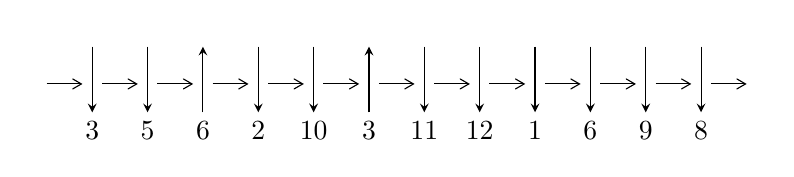
\begin{tikzpicture}[x=20pt, y=17pt]
	% nodes
	\node (C0) at (0, 0) {};
	\node (C1) at (1, 0) {};
	\node (C1U) at (1, +1) {};
	\node (C1D) at (1, -1) {3};

	\node (C2) at (2, 0) {};
	\node (C2U) at (2, +1) {};
	\node (C2D) at (2, -1) {5};

	\node (C3) at (3, 0) {};
	\node (C3U) at (3, +1) {};
	\node (C3D) at (3, -1) {6};

	\node (C4) at (4, 0) {};
	\node (C4U) at (4, +1) {};
	\node (C4D) at (4, -1) {2};

	\node (C5) at (5, 0) {};
	\node (C5U) at (5, +1) {};
	\node (C5D) at (5, -1) {10};

	\node (C6) at (6, 0) {};
	\node (C6U) at (6, +1) {};
	\node (C6D) at (6, -1) {3};

	\node (C7) at (7, 0) {};
	\node (C7U) at (7, +1) {};
	\node (C7D) at (7, -1) {11};

	\node (C8) at (8, 0) {};
	\node (C8U) at (8, +1) {};
	\node (C8D) at (8, -1) {12};

	\node (C9) at (9, 0) {};
	\node (C9U) at (9, +1) {};
	\node (C9D) at (9, -1) {1};

	\node (C10) at (10, 0) {};
	\node (C10U) at (10, +1) {};
	\node (C10D) at (10, -1) {6};

	\node (C11) at (11, 0) {};
	\node (C11U) at (11, +1) {};
	\node (C11D) at (11, -1) {9};

	\node (C12) at (12, 0) {};
	\node (C12U) at (12, +1) {};
	\node (C12D) at (12, -1) {8};
	\node (C13) at (13, 0) {};

	% arrows
	\draw[->,>={angle 60}]
	(C0) edge (C1) (C1) edge (C2) (C2) edge (C3) (C3) edge (C4) (C4) edge (C5) (C5) edge (C6) (C6) edge (C7) (C7) edge (C8) (C8) edge (C9) (C9) edge (C10) (C10) edge (C11) (C11) edge (C12) (C12) edge (C13) ;	\draw[->,>=stealth]
	(C1U) edge (C1D) (C2U) edge (C2D) (C3D) edge (C3U) (C4U) edge (C4D) (C5U) edge (C5D) (C6D) edge (C6U) (C7U) edge (C7D) (C8U) edge (C8D) (C9U) edge (C9D) (C10U) edge (C10D) (C11U) edge (C11D) (C12U) edge (C12D) ;
	\end{tikzpicture} \\
\hhline{~~} \\& 
\textbf{Solving Sequence} \\ \cline{2-2} 
 &
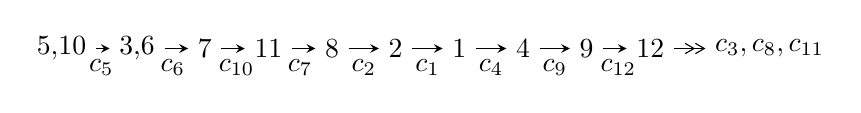
\begin{tikzpicture}[x=23pt, y=7pt]
	% node
	\node (A0) at (-1/8, 0) {5,10};
	\node (A1) at (17/16, 0) {3,6};
	\node (A2) at (17/8, 0) {7};
	\node (A3) at (25/8, 0) {11};
	\node (A4) at (33/8, 0) {8};
	\node (A5) at (41/8, 0) {2};
	\node (A6) at (49/8, 0) {1};
	\node (A7) at (57/8, 0) {4};
	\node (A8) at (65/8, 0) {9};
	\node (A9) at (73/8, 0) {12};
	\node (C1) at (1/2, -1) {$c_{5}$};
	\node (C2) at (13/8, -1) {$c_{6}$};
	\node (C3) at (21/8, -1) {$c_{10}$};
	\node (C4) at (29/8, -1) {$c_{7}$};
	\node (C5) at (37/8, -1) {$c_{2}$};
	\node (C6) at (45/8, -1) {$c_{1}$};
	\node (C7) at (53/8, -1) {$c_{4}$};
	\node (C8) at (61/8, -1) {$c_{9}$};
	\node (C9) at (69/8, -1) {$c_{12}$};
	\node (A10) at (11, 0) {$c_{3},c_{8},c_{11}$};

	% edge
	\draw[->,>=stealth]	
	(A0) edge (A1) (A1) edge (A2) (A2) edge (A3) (A3) edge (A4) (A4) edge (A5) (A5) edge (A6) (A6) edge (A7) (A7) edge (A8) (A8) edge (A9) ;
	\draw[->>,>={angle 60}]	
	(A9) edge (A10);
\end{tikzpicture} \\ 

\end{tabular} \\

\footnotetext{
The image of knot diagram is generated by the software ``\textbf{Draw programme}" developed by Andrew Bartholomew(\url{http://www.layer8.co.uk/maths/draw/index.htm\#Running-draw}), where we modified some parts for our purpose(\url{https://github.com/CATsTAILs/LinksPainter}).
}\phantom \\ \newline 
\centering \textbf{Ideals for irreducible components\footnotemark of $X_{\text{par}}$} 
 
\begin{align*}
I^u_{1}&=\langle 
-1.31243\times10^{79} u^{53}+2.52611\times10^{79} u^{52}+\cdots+3.89056\times10^{79} b+3.47087\times10^{79},\\
\phantom{I^u_{1}}&\phantom{= \langle  }-6.05548\times10^{79} u^{53}+8.73883\times10^{79} u^{52}+\cdots+3.89056\times10^{79} a+1.31119\times10^{80},\;u^{54}-2 u^{53}+\cdots- u+1\rangle \\
I^u_{2}&=\langle 
b+1,\;u^5-4 u^3- u^2+a+4 u+3,\;u^6- u^5-3 u^4+2 u^3+2 u^2+u-1\rangle \\
\\
\end{align*}
\raggedright * 2 irreducible components of $\dim_{\mathbb{C}}=0$, with total 60 representations.\\
\footnotetext{All coefficients of polynomials are rational numbers. But the coefficients are sometimes approximated in decimal forms when there is not enough margin.}
\newpage
\renewcommand{\arraystretch}{1}
\centering \section*{I. $I^u_{1}= \langle -1.31\times10^{79} u^{53}+2.53\times10^{79} u^{52}+\cdots+3.89\times10^{79} b+3.47\times10^{79},\;-6.06\times10^{79} u^{53}+8.74\times10^{79} u^{52}+\cdots+3.89\times10^{79} a+1.31\times10^{80},\;u^{54}-2 u^{53}+\cdots- u+1 \rangle$}
\flushleft \textbf{(i) Arc colorings}\\
\begin{tabular}{m{7pt} m{180pt} m{7pt} m{180pt} }
\flushright $a_{5}=$&$\begin{pmatrix}1\\0\end{pmatrix}$ \\
\flushright $a_{10}=$&$\begin{pmatrix}0\\u\end{pmatrix}$ \\
\flushright $a_{3}=$&$\begin{pmatrix}1.55645 u^{53}-2.24616 u^{52}+\cdots-5.64280 u-3.37019\\0.337337 u^{53}-0.649292 u^{52}+\cdots-1.00166 u-0.892127\end{pmatrix}$ \\
\flushright $a_{6}=$&$\begin{pmatrix}1\\u^2\end{pmatrix}$ \\
\flushright $a_{7}=$&$\begin{pmatrix}0.494692 u^{53}-0.863004 u^{52}+\cdots-1.15347 u-0.702997\\0.0990880 u^{53}-0.268680 u^{52}+\cdots-0.626964 u-0.0224128\end{pmatrix}$ \\
\flushright $a_{11}=$&$\begin{pmatrix}- u\\- u^3+u\end{pmatrix}$ \\
\flushright $a_{8}=$&$\begin{pmatrix}0.356510 u^{53}-0.587357 u^{52}+\cdots-0.776606 u-0.657794\\0.241891 u^{53}-0.521606 u^{52}+\cdots-0.866363 u-0.0668977\end{pmatrix}$ \\
\flushright $a_{2}=$&$\begin{pmatrix}1.89379 u^{53}-2.89546 u^{52}+\cdots-6.64447 u-4.26232\\0.337337 u^{53}-0.649292 u^{52}+\cdots-1.00166 u-0.892127\end{pmatrix}$ \\
\flushright $a_{1}=$&$\begin{pmatrix}0.422066 u^{53}-0.798929 u^{52}+\cdots-1.41212 u-0.599029\\0.0726263 u^{53}-0.0640750 u^{52}+\cdots+0.258652 u-0.103967\end{pmatrix}$ \\
\flushright $a_{4}=$&$\begin{pmatrix}1.61205 u^{53}-2.39082 u^{52}+\cdots-5.95476 u-3.39557\\0.312040 u^{53}-0.627049 u^{52}+\cdots-1.09072 u-0.858664\end{pmatrix}$ \\
\flushright $a_{9}=$&$\begin{pmatrix}0.224414 u^{53}-0.297818 u^{52}+\cdots+1.50104 u-0.620789\\-0.00237699 u^{53}-0.0155895 u^{52}+\cdots+0.993052 u-0.0916897\end{pmatrix}$ \\
\flushright $a_{12}=$&$\begin{pmatrix}-0.0386938 u^{53}+0.107824 u^{52}+\cdots-0.761082 u-0.0321440\\0.281009 u^{53}-0.285348 u^{52}+\cdots+1.09523 u-0.220603\end{pmatrix}$\\&\end{tabular}
\flushleft \textbf{(ii) Obstruction class $= -1$}\\~\\
\flushleft \textbf{(iii) Cusp Shapes $= -7.59111 u^{53}+13.1261 u^{52}+\cdots+13.3633 u-0.108982$}\\~\\
\newpage\renewcommand{\arraystretch}{1}
\flushleft \textbf{(iv) u-Polynomials at the component}\newline \\
\begin{tabular}{m{50pt}|m{274pt}}
Crossings & \hspace{64pt}u-Polynomials at each crossing \\
\hline $$\begin{aligned}c_{1}\end{aligned}$$&$\begin{aligned}
&u^{54}+21 u^{53}+\cdots+622 u+1
\end{aligned}$\\
\hline $$\begin{aligned}c_{2},c_{4}\end{aligned}$$&$\begin{aligned}
&u^{54}-7 u^{53}+\cdots-26 u+1
\end{aligned}$\\
\hline $$\begin{aligned}c_{3},c_{6}\end{aligned}$$&$\begin{aligned}
&u^{54}+7 u^{53}+\cdots+768 u+64
\end{aligned}$\\
\hline $$\begin{aligned}c_{5},c_{10}\end{aligned}$$&$\begin{aligned}
&u^{54}-2 u^{53}+\cdots- u+1
\end{aligned}$\\
\hline $$\begin{aligned}c_{7},c_{9}\end{aligned}$$&$\begin{aligned}
&u^{54}+2 u^{53}+\cdots+141 u+17
\end{aligned}$\\
\hline $$\begin{aligned}c_{8},c_{11},c_{12}\end{aligned}$$&$\begin{aligned}
&u^{54}-2 u^{53}+\cdots+5 u+1
\end{aligned}$\\
\hline
\end{tabular}\\~\\
\newpage\renewcommand{\arraystretch}{1}
\flushleft \textbf{(v) Riley Polynomials at the component}\newline \\
\begin{tabular}{m{50pt}|m{274pt}}
Crossings & \hspace{64pt}Riley Polynomials at each crossing \\
\hline $$\begin{aligned}c_{1}\end{aligned}$$&$\begin{aligned}
&y^{54}+31 y^{53}+\cdots-394862 y+1
\end{aligned}$\\
\hline $$\begin{aligned}c_{2},c_{4}\end{aligned}$$&$\begin{aligned}
&y^{54}-21 y^{53}+\cdots-622 y+1
\end{aligned}$\\
\hline $$\begin{aligned}c_{3},c_{6}\end{aligned}$$&$\begin{aligned}
&y^{54}-39 y^{53}+\cdots-147456 y+4096
\end{aligned}$\\
\hline $$\begin{aligned}c_{5},c_{10}\end{aligned}$$&$\begin{aligned}
&y^{54}-14 y^{53}+\cdots-13 y+1
\end{aligned}$\\
\hline $$\begin{aligned}c_{7},c_{9}\end{aligned}$$&$\begin{aligned}
&y^{54}-26 y^{53}+\cdots-1997 y+289
\end{aligned}$\\
\hline $$\begin{aligned}c_{8},c_{11},c_{12}\end{aligned}$$&$\begin{aligned}
&y^{54}+46 y^{53}+\cdots-13 y+1
\end{aligned}$\\
\hline
\end{tabular}\\~\\
\newpage\flushleft \textbf{(vi) Complex Volumes and Cusp Shapes}
$$\begin{array}{c|c|c}  
\text{Solutions to }I^u_{1}& \I (\text{vol} + \sqrt{-1}CS) & \text{Cusp shape}\\
 \hline 
\begin{aligned}
u &= -0.768246 + 0.418674 I \\
a &= \phantom{-}0.229316 - 1.287030 I \\
b &= -0.920583 + 0.946817 I\end{aligned}
 & \phantom{-}0.59137 + 6.88514 I & -9.74374 - 8.93563 I \\ \hline\begin{aligned}
u &= -0.768246 - 0.418674 I \\
a &= \phantom{-}0.229316 + 1.287030 I \\
b &= -0.920583 - 0.946817 I\end{aligned}
 & \phantom{-}0.59137 - 6.88514 I & -9.74374 + 8.93563 I \\ \hline\begin{aligned}
u &= \phantom{-}0.607809 + 0.618855 I \\
a &= \phantom{-}0.260894 + 0.992870 I \\
b &= -0.199900 - 0.710236 I\end{aligned}
 & \phantom{-}3.57906 - 1.48496 I & -4.05718 + 4.03244 I \\ \hline\begin{aligned}
u &= \phantom{-}0.607809 - 0.618855 I \\
a &= \phantom{-}0.260894 - 0.992870 I \\
b &= -0.199900 + 0.710236 I\end{aligned}
 & \phantom{-}3.57906 + 1.48496 I & -4.05718 - 4.03244 I \\ \hline\begin{aligned}
u &= -0.764967 + 0.849835 I \\
a &= -0.290324 - 0.846955 I \\
b &= \phantom{-}0.429432 + 1.086500 I\end{aligned}
 & \phantom{-}1.86993 + 4.42374 I & \phantom{-0.000000 } 0 \\ \hline\begin{aligned}
u &= -0.764967 - 0.849835 I \\
a &= -0.290324 + 0.846955 I \\
b &= \phantom{-}0.429432 - 1.086500 I\end{aligned}
 & \phantom{-}1.86993 - 4.42374 I & \phantom{-0.000000 } 0 \\ \hline\begin{aligned}
u &= \phantom{-}0.704848 + 0.923652 I \\
a &= -0.256437 + 0.652141 I \\
b &= \phantom{-}0.534153 - 0.864717 I\end{aligned}
 & \phantom{-}3.77813 - 0.69821 I & \phantom{-0.000000 } 0 \\ \hline\begin{aligned}
u &= \phantom{-}0.704848 - 0.923652 I \\
a &= -0.256437 - 0.652141 I \\
b &= \phantom{-}0.534153 + 0.864717 I\end{aligned}
 & \phantom{-}3.77813 + 0.69821 I & \phantom{-0.000000 } 0 \\ \hline\begin{aligned}
u &= \phantom{-}0.746032 + 0.376084 I \\
a &= \phantom{-}0.208695 + 1.272420 I \\
b &= -1.000010 - 0.815508 I\end{aligned}
 & -3.84826 - 3.29989 I & -15.7501 + 7.0561 I \\ \hline\begin{aligned}
u &= \phantom{-}0.746032 - 0.376084 I \\
a &= \phantom{-}0.208695 - 1.272420 I \\
b &= -1.000010 + 0.815508 I\end{aligned}
 & -3.84826 + 3.29989 I & -15.7501 - 7.0561 I\\
 \hline 
 \end{array}$$\newpage$$\begin{array}{c|c|c}  
\text{Solutions to }I^u_{1}& \I (\text{vol} + \sqrt{-1}CS) & \text{Cusp shape}\\
 \hline 
\begin{aligned}
u &= \phantom{-}0.803876 + 0.851386 I \\
a &= -0.369782 + 0.893548 I \\
b &= \phantom{-}0.480584 - 1.193560 I\end{aligned}
 & \phantom{-}6.92007 - 8.14255 I & \phantom{-0.000000 } 0 \\ \hline\begin{aligned}
u &= \phantom{-}0.803876 - 0.851386 I \\
a &= -0.369782 - 0.893548 I \\
b &= \phantom{-}0.480584 + 1.193560 I\end{aligned}
 & \phantom{-}6.92007 + 8.14255 I & \phantom{-0.000000 } 0 \\ \hline\begin{aligned}
u &= -0.741661 + 0.299782 I \\
a &= \phantom{-}0.129845 - 1.191170 I \\
b &= -1.173070 + 0.667650 I\end{aligned}
 & -0.523210 - 0.060545 I & -12.38307 - 2.35064 I \\ \hline\begin{aligned}
u &= -0.741661 - 0.299782 I \\
a &= \phantom{-}0.129845 + 1.191170 I \\
b &= -1.173070 - 0.667650 I\end{aligned}
 & -0.523210 + 0.060545 I & -12.38307 + 2.35064 I \\ \hline\begin{aligned}
u &= \phantom{-}0.773740 + 0.056042 I \\
a &= -0.048323 + 0.281192 I \\
b &= -1.57214 - 0.14784 I\end{aligned}
 & -1.63990 - 3.52551 I & -13.9655 + 3.9216 I \\ \hline\begin{aligned}
u &= \phantom{-}0.773740 - 0.056042 I \\
a &= -0.048323 - 0.281192 I \\
b &= -1.57214 + 0.14784 I\end{aligned}
 & -1.63990 + 3.52551 I & -13.9655 - 3.9216 I \\ \hline\begin{aligned}
u &= -0.761194\phantom{ +0.000000I} \\
a &= -0.126584\phantom{ +0.000000I} \\
b &= -1.55203\phantom{ +0.000000I}\end{aligned}
 & -5.56883\phantom{ +0.000000I} & -19.2640\phantom{ +0.000000I} \\ \hline\begin{aligned}
u &= -0.801458 + 0.970429 I \\
a &= -0.477469 - 0.628269 I \\
b &= \phantom{-}0.772246 + 0.988987 I\end{aligned}
 & \phantom{-}10.54700 + 0.04212 I & \phantom{-0.000000 } 0 \\ \hline\begin{aligned}
u &= -0.801458 - 0.970429 I \\
a &= -0.477469 + 0.628269 I \\
b &= \phantom{-}0.772246 - 0.988987 I\end{aligned}
 & \phantom{-}10.54700 - 0.04212 I & \phantom{-0.000000 } 0 \\ \hline\begin{aligned}
u &= \phantom{-}1.029720 + 0.727275 I \\
a &= \phantom{-}0.864484 - 1.045500 I \\
b &= \phantom{-}0.745526 + 0.764163 I\end{aligned}
 & \phantom{-}6.18806 + 2.15434 I & \phantom{-0.000000 } 0\\
 \hline 
 \end{array}$$\newpage$$\begin{array}{c|c|c}  
\text{Solutions to }I^u_{1}& \I (\text{vol} + \sqrt{-1}CS) & \text{Cusp shape}\\
 \hline 
\begin{aligned}
u &= \phantom{-}1.029720 - 0.727275 I \\
a &= \phantom{-}0.864484 + 1.045500 I \\
b &= \phantom{-}0.745526 - 0.764163 I\end{aligned}
 & \phantom{-}6.18806 - 2.15434 I & \phantom{-0.000000 } 0 \\ \hline\begin{aligned}
u &= \phantom{-}0.680095 + 1.079720 I \\
a &= -0.295388 + 0.394253 I \\
b &= \phantom{-}0.744693 - 0.637616 I\end{aligned}
 & \phantom{-}3.23226 - 0.56101 I & \phantom{-0.000000 } 0 \\ \hline\begin{aligned}
u &= \phantom{-}0.680095 - 1.079720 I \\
a &= -0.295388 - 0.394253 I \\
b &= \phantom{-}0.744693 + 0.637616 I\end{aligned}
 & \phantom{-}3.23226 + 0.56101 I & \phantom{-0.000000 } 0 \\ \hline\begin{aligned}
u &= -1.094030 + 0.729061 I \\
a &= \phantom{-}0.716084 + 0.962560 I \\
b &= \phantom{-}0.826123 - 0.670841 I\end{aligned}
 & \phantom{-}0.83207 + 1.55401 I & \phantom{-0.000000 } 0 \\ \hline\begin{aligned}
u &= -1.094030 - 0.729061 I \\
a &= \phantom{-}0.716084 - 0.962560 I \\
b &= \phantom{-}0.826123 + 0.670841 I\end{aligned}
 & \phantom{-}0.83207 - 1.55401 I & \phantom{-0.000000 } 0 \\ \hline\begin{aligned}
u &= \phantom{-}0.545482 + 0.387512 I \\
a &= \phantom{-}1.49627 + 0.17225 I \\
b &= -0.109480 + 0.221560 I\end{aligned}
 & \phantom{-}3.26577 - 2.10907 I & -4.57255 + 4.21158 I \\ \hline\begin{aligned}
u &= \phantom{-}0.545482 - 0.387512 I \\
a &= \phantom{-}1.49627 - 0.17225 I \\
b &= -0.109480 - 0.221560 I\end{aligned}
 & \phantom{-}3.26577 + 2.10907 I & -4.57255 - 4.21158 I \\ \hline\begin{aligned}
u &= -0.549686 + 0.379087 I \\
a &= \phantom{-}0.41820 - 1.65690 I \\
b &= -0.756383 + 0.350743 I\end{aligned}
 & -0.98992 + 1.28097 I & -8.23381 - 4.95312 I \\ \hline\begin{aligned}
u &= -0.549686 - 0.379087 I \\
a &= \phantom{-}0.41820 + 1.65690 I \\
b &= -0.756383 - 0.350743 I\end{aligned}
 & -0.98992 - 1.28097 I & -8.23381 + 4.95312 I \\ \hline\begin{aligned}
u &= -0.765980 + 1.114890 I \\
a &= -0.423959 - 0.343278 I \\
b &= \phantom{-}0.903717 + 0.672502 I\end{aligned}
 & \phantom{-}0.58680 - 3.64832 I & \phantom{-0.000000 } 0\\
 \hline 
 \end{array}$$\newpage$$\begin{array}{c|c|c}  
\text{Solutions to }I^u_{1}& \I (\text{vol} + \sqrt{-1}CS) & \text{Cusp shape}\\
 \hline 
\begin{aligned}
u &= -0.765980 - 1.114890 I \\
a &= -0.423959 + 0.343278 I \\
b &= \phantom{-}0.903717 - 0.672502 I\end{aligned}
 & \phantom{-}0.58680 + 3.64832 I & \phantom{-0.000000 } 0 \\ \hline\begin{aligned}
u &= -1.072810 + 0.850554 I \\
a &= \phantom{-}0.521225 + 1.271540 I \\
b &= \phantom{-}1.038160 - 0.833697 I\end{aligned}
 & \phantom{-}9.68000 + 6.67132 I & \phantom{-0.000000 } 0 \\ \hline\begin{aligned}
u &= -1.072810 - 0.850554 I \\
a &= \phantom{-}0.521225 - 1.271540 I \\
b &= \phantom{-}1.038160 + 0.833697 I\end{aligned}
 & \phantom{-}9.68000 - 6.67132 I & \phantom{-0.000000 } 0 \\ \hline\begin{aligned}
u &= \phantom{-}0.809181 + 1.110190 I \\
a &= -0.498165 + 0.338281 I \\
b &= \phantom{-}0.978433 - 0.715727 I\end{aligned}
 & \phantom{-}5.47300 + 7.77762 I & \phantom{-0.000000 } 0 \\ \hline\begin{aligned}
u &= \phantom{-}0.809181 - 1.110190 I \\
a &= -0.498165 - 0.338281 I \\
b &= \phantom{-}0.978433 + 0.715727 I\end{aligned}
 & \phantom{-}5.47300 - 7.77762 I & \phantom{-0.000000 } 0 \\ \hline\begin{aligned}
u &= -0.355157 + 0.506837 I \\
a &= \phantom{-}3.09166 - 1.48155 I \\
b &= -0.790878 - 0.242839 I\end{aligned}
 & \phantom{-}1.75113 - 3.66412 I & -7.58424 - 2.09874 I \\ \hline\begin{aligned}
u &= -0.355157 - 0.506837 I \\
a &= \phantom{-}3.09166 + 1.48155 I \\
b &= -0.790878 + 0.242839 I\end{aligned}
 & \phantom{-}1.75113 + 3.66412 I & -7.58424 + 2.09874 I \\ \hline\begin{aligned}
u &= \phantom{-}1.127980 + 0.801217 I \\
a &= \phantom{-}0.525545 - 1.040990 I \\
b &= \phantom{-}0.975741 + 0.675989 I\end{aligned}
 & \phantom{-}2.46104 - 5.73021 I & \phantom{-0.000000 } 0 \\ \hline\begin{aligned}
u &= \phantom{-}1.127980 - 0.801217 I \\
a &= \phantom{-}0.525545 + 1.040990 I \\
b &= \phantom{-}0.975741 - 0.675989 I\end{aligned}
 & \phantom{-}2.46104 + 5.73021 I & \phantom{-0.000000 } 0 \\ \hline\begin{aligned}
u &= \phantom{-}1.13900 + 0.87943 I \\
a &= \phantom{-}0.314802 - 1.138340 I \\
b &= \phantom{-}1.146120 + 0.686785 I\end{aligned}
 & \phantom{-}1.85511 - 6.51126 I & \phantom{-0.000000 } 0\\
 \hline 
 \end{array}$$\newpage$$\begin{array}{c|c|c}  
\text{Solutions to }I^u_{1}& \I (\text{vol} + \sqrt{-1}CS) & \text{Cusp shape}\\
 \hline 
\begin{aligned}
u &= \phantom{-}1.13900 - 0.87943 I \\
a &= \phantom{-}0.314802 + 1.138340 I \\
b &= \phantom{-}1.146120 - 0.686785 I\end{aligned}
 & \phantom{-}1.85511 + 6.51126 I & \phantom{-0.000000 } 0 \\ \hline\begin{aligned}
u &= \phantom{-}1.11062 + 0.91730 I \\
a &= \phantom{-}0.232119 - 1.286790 I \\
b &= \phantom{-}1.24453 + 0.76770 I\end{aligned}
 & \phantom{-}4.4865 - 15.0788 I & \phantom{-0.000000 } 0 \\ \hline\begin{aligned}
u &= \phantom{-}1.11062 - 0.91730 I \\
a &= \phantom{-}0.232119 + 1.286790 I \\
b &= \phantom{-}1.24453 - 0.76770 I\end{aligned}
 & \phantom{-}4.4865 + 15.0788 I & \phantom{-0.000000 } 0 \\ \hline\begin{aligned}
u &= -1.12423 + 0.90674 I \\
a &= \phantom{-}0.249320 + 1.222810 I \\
b &= \phantom{-}1.21483 - 0.72751 I\end{aligned}
 & -0.55203 + 10.91430 I & \phantom{-0.000000 } 0 \\ \hline\begin{aligned}
u &= -1.12423 - 0.90674 I \\
a &= \phantom{-}0.249320 - 1.222810 I \\
b &= \phantom{-}1.21483 + 0.72751 I\end{aligned}
 & -0.55203 - 10.91430 I & \phantom{-0.000000 } 0 \\ \hline\begin{aligned}
u &= \phantom{-}0.298615 + 0.438132 I \\
a &= \phantom{-}3.44332 + 2.65285 I \\
b &= -0.886190 + 0.122203 I\end{aligned}
 & -2.63664 + 0.46428 I & -17.5611 + 8.2084 I \\ \hline\begin{aligned}
u &= \phantom{-}0.298615 - 0.438132 I \\
a &= \phantom{-}3.44332 - 2.65285 I \\
b &= -0.886190 - 0.122203 I\end{aligned}
 & -2.63664 - 0.46428 I & -17.5611 - 8.2084 I \\ \hline\begin{aligned}
u &= -0.158468 + 0.454530 I \\
a &= \phantom{-}5.77902 - 2.31620 I \\
b &= -1.028880 - 0.101463 I\end{aligned}
 & \phantom{-}1.11313 + 2.46535 I & \phantom{-}1.5488 - 21.3906 I \\ \hline\begin{aligned}
u &= -0.158468 - 0.454530 I \\
a &= \phantom{-}5.77902 + 2.31620 I \\
b &= -1.028880 + 0.101463 I\end{aligned}
 & \phantom{-}1.11313 - 2.46535 I & \phantom{-}1.5488 + 21.3906 I \\ \hline\begin{aligned}
u &= -0.455910\phantom{ +0.000000I} \\
a &= \phantom{-}1.15202\phantom{ +0.000000I} \\
b &= \phantom{-}0.0398888\phantom{ +0.000000I}\end{aligned}
 & -0.785514\phantom{ +0.000000I} & -12.5200\phantom{ +0.000000I}\\
 \hline 
 \end{array}$$\newpage$$\begin{array}{c|c|c}  
\text{Solutions to }I^u_{1}& \I (\text{vol} + \sqrt{-1}CS) & \text{Cusp shape}\\
 \hline 
\begin{aligned}
u &= \phantom{-}0.453888\phantom{ +0.000000I} \\
a &= -3.16883\phantom{ +0.000000I} \\
b &= -1.08168\phantom{ +0.000000I}\end{aligned}
 & -2.16763\phantom{ +0.000000I} & \phantom{-}5.07630\phantom{ +0.000000I} \\ \hline\begin{aligned}
u &= -1.61778 + 0.14927 I \\
a &= \phantom{-}0.501712 + 0.090012 I \\
b &= \phantom{-}0.800121 - 0.055050 I\end{aligned}
 & -4.90969 + 4.71375 I & \phantom{-0.000000 } 0 \\ \hline\begin{aligned}
u &= -1.61778 - 0.14927 I \\
a &= \phantom{-}0.501712 - 0.090012 I \\
b &= \phantom{-}0.800121 + 0.055050 I\end{aligned}
 & -4.90969 - 4.71375 I & \phantom{-0.000000 } 0 \\ \hline\begin{aligned}
u &= \phantom{-}1.63817\phantom{ +0.000000I} \\
a &= \phantom{-}0.498085\phantom{ +0.000000I} \\
b &= \phantom{-}0.800035\phantom{ +0.000000I}\end{aligned}
 & -8.87320\phantom{ +0.000000I} & \phantom{-0.000000 } 0\\
 \hline 
 \end{array}$$\newpage\newpage\renewcommand{\arraystretch}{1}
\centering \section*{II. $I^u_{2}= \langle b+1,\;u^5-4 u^3- u^2+a+4 u+3,\;u^6- u^5-3 u^4+2 u^3+2 u^2+u-1 \rangle$}
\flushleft \textbf{(i) Arc colorings}\\
\begin{tabular}{m{7pt} m{180pt} m{7pt} m{180pt} }
\flushright $a_{5}=$&$\begin{pmatrix}1\\0\end{pmatrix}$ \\
\flushright $a_{10}=$&$\begin{pmatrix}0\\u\end{pmatrix}$ \\
\flushright $a_{3}=$&$\begin{pmatrix}- u^5+4 u^3+u^2-4 u-3\\-1\end{pmatrix}$ \\
\flushright $a_{6}=$&$\begin{pmatrix}1\\u^2\end{pmatrix}$ \\
\flushright $a_{7}=$&$\begin{pmatrix}1\\u^2\end{pmatrix}$ \\
\flushright $a_{11}=$&$\begin{pmatrix}- u\\- u^3+u\end{pmatrix}$ \\
\flushright $a_{8}=$&$\begin{pmatrix}- u^2+1\\- u^4+2 u^2\end{pmatrix}$ \\
\flushright $a_{2}=$&$\begin{pmatrix}- u^5+4 u^3+u^2-4 u-4\\-1\end{pmatrix}$ \\
\flushright $a_{1}=$&$\begin{pmatrix}-1\\0\end{pmatrix}$ \\
\flushright $a_{4}=$&$\begin{pmatrix}- u^5+4 u^3+u^2-4 u-3\\-1\end{pmatrix}$ \\
\flushright $a_{9}=$&$\begin{pmatrix}u\\u\end{pmatrix}$ \\
\flushright $a_{12}=$&$\begin{pmatrix}u^5-2 u^3- u\\u^5-3 u^3+u\end{pmatrix}$\\&\end{tabular}
\flushleft \textbf{(ii) Obstruction class $= 1$}\\~\\
\flushleft \textbf{(iii) Cusp Shapes $= -7 u^5+3 u^4+27 u^3-5 u^2-24 u-26$}\\~\\
\newpage\renewcommand{\arraystretch}{1}
\flushleft \textbf{(iv) u-Polynomials at the component}\newline \\
\begin{tabular}{m{50pt}|m{274pt}}
Crossings & \hspace{64pt}u-Polynomials at each crossing \\
\hline $$\begin{aligned}c_{1},c_{2}\end{aligned}$$&$\begin{aligned}
&(u-1)^6
\end{aligned}$\\
\hline $$\begin{aligned}c_{3},c_{6}\end{aligned}$$&$\begin{aligned}
&u^6
\end{aligned}$\\
\hline $$\begin{aligned}c_{4}\end{aligned}$$&$\begin{aligned}
&(u+1)^6
\end{aligned}$\\
\hline $$\begin{aligned}c_{5},c_{7},c_{9}\end{aligned}$$&$\begin{aligned}
&u^6- u^5-3 u^4+2 u^3+2 u^2+u-1
\end{aligned}$\\
\hline $$\begin{aligned}c_{8}\end{aligned}$$&$\begin{aligned}
&u^6+u^5+3 u^4+2 u^3+2 u^2+u-1
\end{aligned}$\\
\hline $$\begin{aligned}c_{10}\end{aligned}$$&$\begin{aligned}
&u^6+u^5-3 u^4-2 u^3+2 u^2- u-1
\end{aligned}$\\
\hline $$\begin{aligned}c_{11},c_{12}\end{aligned}$$&$\begin{aligned}
&u^6- u^5+3 u^4-2 u^3+2 u^2- u-1
\end{aligned}$\\
\hline
\end{tabular}\\~\\
\newpage\renewcommand{\arraystretch}{1}
\flushleft \textbf{(v) Riley Polynomials at the component}\newline \\
\begin{tabular}{m{50pt}|m{274pt}}
Crossings & \hspace{64pt}Riley Polynomials at each crossing \\
\hline $$\begin{aligned}c_{1},c_{2},c_{4}\end{aligned}$$&$\begin{aligned}
&(y-1)^6
\end{aligned}$\\
\hline $$\begin{aligned}c_{3},c_{6}\end{aligned}$$&$\begin{aligned}
&y^6
\end{aligned}$\\
\hline $$\begin{aligned}c_{5},c_{7},c_{9}\\c_{10}\end{aligned}$$&$\begin{aligned}
&y^6-7 y^5+17 y^4-16 y^3+6 y^2-5 y+1
\end{aligned}$\\
\hline $$\begin{aligned}c_{8},c_{11},c_{12}\end{aligned}$$&$\begin{aligned}
&y^6+5 y^5+9 y^4+4 y^3-6 y^2-5 y+1
\end{aligned}$\\
\hline
\end{tabular}\\~\\
\newpage\flushleft \textbf{(vi) Complex Volumes and Cusp Shapes}
$$\begin{array}{c|c|c}  
\text{Solutions to }I^u_{2}& \I (\text{vol} + \sqrt{-1}CS) & \text{Cusp shape}\\
 \hline 
\begin{aligned}
u &= -0.493180 + 0.575288 I \\
a &= \phantom{-}0.26610 - 1.72116 I \\
b &= -1.00000\phantom{ +0.000000I}\end{aligned}
 & \phantom{-}1.31531 + 1.97241 I & -5.36986 - 2.86834 I \\ \hline\begin{aligned}
u &= -0.493180 - 0.575288 I \\
a &= \phantom{-}0.26610 + 1.72116 I \\
b &= -1.00000\phantom{ +0.000000I}\end{aligned}
 & \phantom{-}1.31531 - 1.97241 I & -5.36986 + 2.86834 I \\ \hline\begin{aligned}
u &= \phantom{-}0.483672\phantom{ +0.000000I} \\
a &= -4.27462\phantom{ +0.000000I} \\
b &= -1.00000\phantom{ +0.000000I}\end{aligned}
 & -2.38379\phantom{ +0.000000I} & -35.7440\phantom{ +0.000000I} \\ \hline\begin{aligned}
u &= \phantom{-}1.52087 + 0.16310 I \\
a &= -0.417699 + 0.090629 I \\
b &= -1.00000\phantom{ +0.000000I}\end{aligned}
 & -5.34051 - 4.59213 I & -17.7291 + 1.0120 I \\ \hline\begin{aligned}
u &= \phantom{-}1.52087 - 0.16310 I \\
a &= -0.417699 - 0.090629 I \\
b &= -1.00000\phantom{ +0.000000I}\end{aligned}
 & -5.34051 + 4.59213 I & -17.7291 - 1.0120 I \\ \hline\begin{aligned}
u &= -1.53904\phantom{ +0.000000I} \\
a &= -0.422181\phantom{ +0.000000I} \\
b &= -1.00000\phantom{ +0.000000I}\end{aligned}
 & -9.30502\phantom{ +0.000000I} & -22.0580\phantom{ +0.000000I}\\
 \hline 
 \end{array}$$\newpage
\newpage\renewcommand{\arraystretch}{1}
\centering \section*{ III. u-Polynomials}
\begin{tabular}{m{50pt}|m{274pt}}
Crossings & \hspace{64pt}u-Polynomials at each crossing \\
\hline $$\begin{aligned}c_{1}\end{aligned}$$&$\begin{aligned}
&((u-1)^6)(u^{54}+21 u^{53}+\cdots+622 u+1)
\end{aligned}$\\
\hline $$\begin{aligned}c_{2}\end{aligned}$$&$\begin{aligned}
&((u-1)^6)(u^{54}-7 u^{53}+\cdots-26 u+1)
\end{aligned}$\\
\hline $$\begin{aligned}c_{3},c_{6}\end{aligned}$$&$\begin{aligned}
&u^6(u^{54}+7 u^{53}+\cdots+768 u+64)
\end{aligned}$\\
\hline $$\begin{aligned}c_{4}\end{aligned}$$&$\begin{aligned}
&((u+1)^6)(u^{54}-7 u^{53}+\cdots-26 u+1)
\end{aligned}$\\
\hline $$\begin{aligned}c_{5}\end{aligned}$$&$\begin{aligned}
&(u^6- u^5-3 u^4+2 u^3+2 u^2+u-1)(u^{54}-2 u^{53}+\cdots- u+1)
\end{aligned}$\\
\hline $$\begin{aligned}c_{7},c_{9}\end{aligned}$$&$\begin{aligned}
&(u^6- u^5-3 u^4+2 u^3+2 u^2+u-1)(u^{54}+2 u^{53}+\cdots+141 u+17)
\end{aligned}$\\
\hline $$\begin{aligned}c_{8}\end{aligned}$$&$\begin{aligned}
&(u^6+u^5+3 u^4+2 u^3+2 u^2+u-1)(u^{54}-2 u^{53}+\cdots+5 u+1)
\end{aligned}$\\
\hline $$\begin{aligned}c_{10}\end{aligned}$$&$\begin{aligned}
&(u^6+u^5-3 u^4-2 u^3+2 u^2- u-1)(u^{54}-2 u^{53}+\cdots- u+1)
\end{aligned}$\\
\hline $$\begin{aligned}c_{11},c_{12}\end{aligned}$$&$\begin{aligned}
&(u^6- u^5+3 u^4-2 u^3+2 u^2- u-1)(u^{54}-2 u^{53}+\cdots+5 u+1)
\end{aligned}$\\
\hline
\end{tabular}\newpage\renewcommand{\arraystretch}{1}
\centering \section*{ IV. Riley Polynomials}
\begin{tabular}{m{50pt}|m{274pt}}
Crossings & \hspace{64pt}Riley Polynomials at each crossing \\
\hline $$\begin{aligned}c_{1}\end{aligned}$$&$\begin{aligned}
&((y-1)^6)(y^{54}+31 y^{53}+\cdots-394862 y+1)
\end{aligned}$\\
\hline $$\begin{aligned}c_{2},c_{4}\end{aligned}$$&$\begin{aligned}
&((y-1)^6)(y^{54}-21 y^{53}+\cdots-622 y+1)
\end{aligned}$\\
\hline $$\begin{aligned}c_{3},c_{6}\end{aligned}$$&$\begin{aligned}
&y^6(y^{54}-39 y^{53}+\cdots-147456 y+4096)
\end{aligned}$\\
\hline $$\begin{aligned}c_{5},c_{10}\end{aligned}$$&$\begin{aligned}
&(y^6-7 y^5+\cdots-5 y+1)(y^{54}-14 y^{53}+\cdots-13 y+1)
\end{aligned}$\\
\hline $$\begin{aligned}c_{7},c_{9}\end{aligned}$$&$\begin{aligned}
&(y^6-7 y^5+17 y^4-16 y^3+6 y^2-5 y+1)\\
&\cdot(y^{54}-26 y^{53}+\cdots-1997 y+289)
\end{aligned}$\\
\hline $$\begin{aligned}c_{8},c_{11},c_{12}\end{aligned}$$&$\begin{aligned}
&(y^6+5 y^5+\cdots-5 y+1)(y^{54}+46 y^{53}+\cdots-13 y+1)
\end{aligned}$\\
\hline
\end{tabular}
\vskip 2pc
\end{document}